\documentclass[10pt]{article}
\usepackage[margin=0.85in]{geometry}
\usepackage{amsmath,amssymb,booktabs,graphicx,caption}
\usepackage[hidelinks]{hyperref}
\captionsetup{font=small}
\setlength{\tabcolsep}{4pt}

\title{What the gap and the trial overlap do to the filter itself:\\ two-qubit gates, $R_z$ rotations and evolution time}
\author{Data report for the filter-pipeline paper}
\date{\today}

\begin{document}
\maketitle

\noindent This report looks at the filter on its own, with the trial-state circuit excluded. It uses the same
222 cases as the gap/overlap report: open $J_1$--$J_2$ chains with $N=8$--14, the gap $\Delta$ held fixed
across $N$ by tuning $J_2$, and the overlap $\gamma$ held fixed by a sublattice rotation of a $\chi=16$ MPS.
For each case and each filter (dyadic SBC, QETU), it reports
\begin{itemize}
\item \textbf{CNOTs} and \textbf{arbitrary $R_z$ rotations} of the Trotterised filter circuit,
\item the \textbf{evolution time} $T$: the total Hamiltonian simulation time over all pulses or queries, in physical
units $1/J_1$,
\item the \textbf{Trotter step} $dt$ and the number of second-order Strang steps,
\end{itemize}
both \emph{per shot} (one run of the circuit) and \emph{per success} (divided by the success probability $p$).
\emph{Measured} means the cheapest circuit that reaches $1-F\le\varepsilon$ in exact state-vector simulation.
\emph{Certified} means the circuit Theorem~1 guarantees, with exact energies. Counts are rebuilt from the stored
schedules by \texttt{derive\_gapov\_filter.py}, which checks that it reproduces every stored measured total.
Everything below is generated by \texttt{gapov\_report/make\_report\_filter.py}.

\section{The short answer}

\begin{itemize}
\item \textbf{The gap sets the circuit; the overlap sets how often you run it.} Per shot, the overlap enters only
through the logarithm $L=\ln[(1-\gamma)/(\gamma\varepsilon)]$, while the gap enters as a power. Lowering $\gamma$
thirtyfold (0.9 to 0.03) at fixed gap raises the measured CNOTs per shot by only 1.2--3.0$\times$ (dyadic) and
1.5--2.9$\times$ (QETU). Closing the gap by just 1.8$\times$ (0.55 to 0.30) at fixed overlap raises them by 2.7--4.4$\times$
(dyadic) and 1.7--1.9$\times$ (QETU). The overlap's real cost is the repetition: the expected cost per success carries a
further factor $1/p\approx1/\gamma$.
\item \textbf{Evolution time does not depend on $N$} at a fixed gap and overlap. It follows
$T\propto L/\Delta$, the time needed to resolve the gap with log-accuracy, for both filters. CNOTs and $R_z$ grow
with $N$ only through the cost of each Trotter step (and, for QETU, through the step length).
\item \textbf{$R_z$ and CNOTs scale identically.} Every second-order step has a fixed mix of Pauli rotations and
CNOTs, so $R_z/\text{CNOT}=0.25$ in every case. Everything said about CNOTs holds for $R_z$, and so for the
$T$-count in a fault-tolerant setting.
\item \textbf{The certificate gets the filter length right but not the Trotter step.} The certified evolution time is
only 1.2--3$\times$ (median 2.0$\times$) the measured one for dyadic and 1.0--2$\times$ (median 1.3$\times$) for QETU. Its Trotter steps, however, are
26.2--339$\times$ (median 89.4$\times$) and 7.3--68$\times$ (median 19.2$\times$) more numerous. Almost all of the certificate's overhead is in the a-priori Trotter
bound.
\end{itemize}

\section{Study A: gap fixed, overlap varied}

\begin{figure}[h]\centering
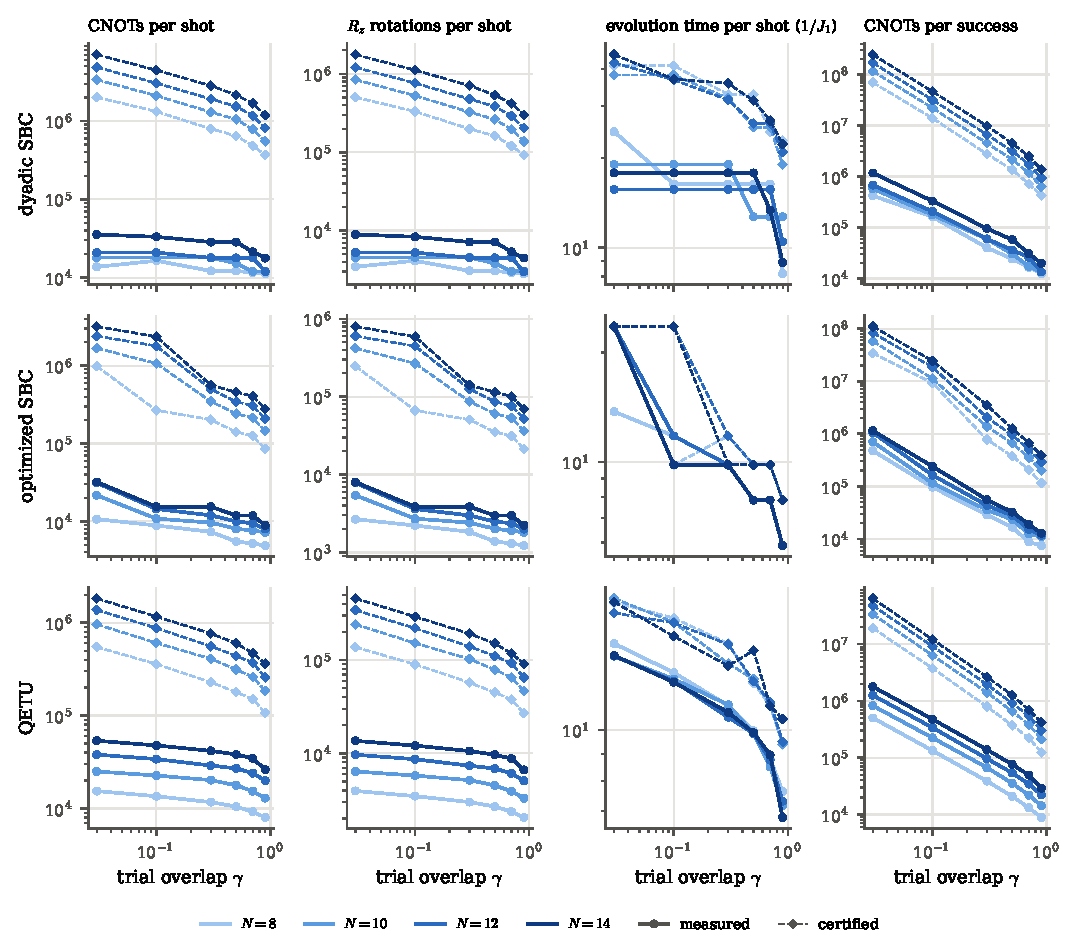
\includegraphics[width=\linewidth]{figs/fig_filter_A.pdf}
\caption{Filter-only resources at $\Delta=0.40$ and $\varepsilon=10^{-3}$ against the trial overlap. Top: dyadic
SBC. Bottom: QETU. Solid: measured. Dashed: certified. The first three columns are per shot; the last is per
success.}\label{fig:A}
\end{figure}

Per shot, the overlap barely matters (Fig.~\ref{fig:A}, first three columns). Across all $N$ and $\varepsilon$, going
from $\gamma=0.9$ to 0.03 raises the measured per-shot filter by:
\begin{center}\small
\begin{tabular}{lcc}\toprule
 & CNOTs (and $R_z$) per shot & evolution time per shot \\\midrule
dyadic, measured & 1.2--3.0$\times$ & 1.5--3.0$\times$ \\
QETU, measured & 1.5--2.9$\times$ & 1.5--2.9$\times$ \\
dyadic, certified & 4.6--9.4$\times$ & 1.5--3.0$\times$ \\
QETU, certified & 4.2--7.1$\times$ & 1.5--2.5$\times$ \\
\bottomrule\end{tabular}
\end{center}
That is what the logarithm predicts. Going from $\gamma=0.9$ to 0.03 raises $(1-\gamma)/\gamma$ by about 290$\times$, which adds only
$\ln 290\approx5.7$ to $L$. Across these cases $L$ runs from about 2 to 13. The filter must suppress the excited weight by $\eta^2=\gamma\varepsilon/(1-\gamma)$, so a worse
trial asks for only a few more powers of the filter.

The dyadic measured time moves in steps, not smoothly, because the ladder $(K,r)$ can only grow by whole
pulses. A worse trial often needs no extra pulse at all.

The certified CNOTs respond more to $\gamma$ than the measured ones (4--9$\times$ against 1--3$\times$). This is
not because the certified filter is longer: its time grows by the same 1.5--3$\times$. It is because the
certified Trotter step must also shrink as the total time grows (Section~\ref{sec:mech}).

Per success (last column), $\gamma$ enters as a power: every curve falls roughly as $1/\gamma$. Here the overlap
dominates.

\section{Study B: overlap fixed, gap varied}

\begin{figure}[h]\centering
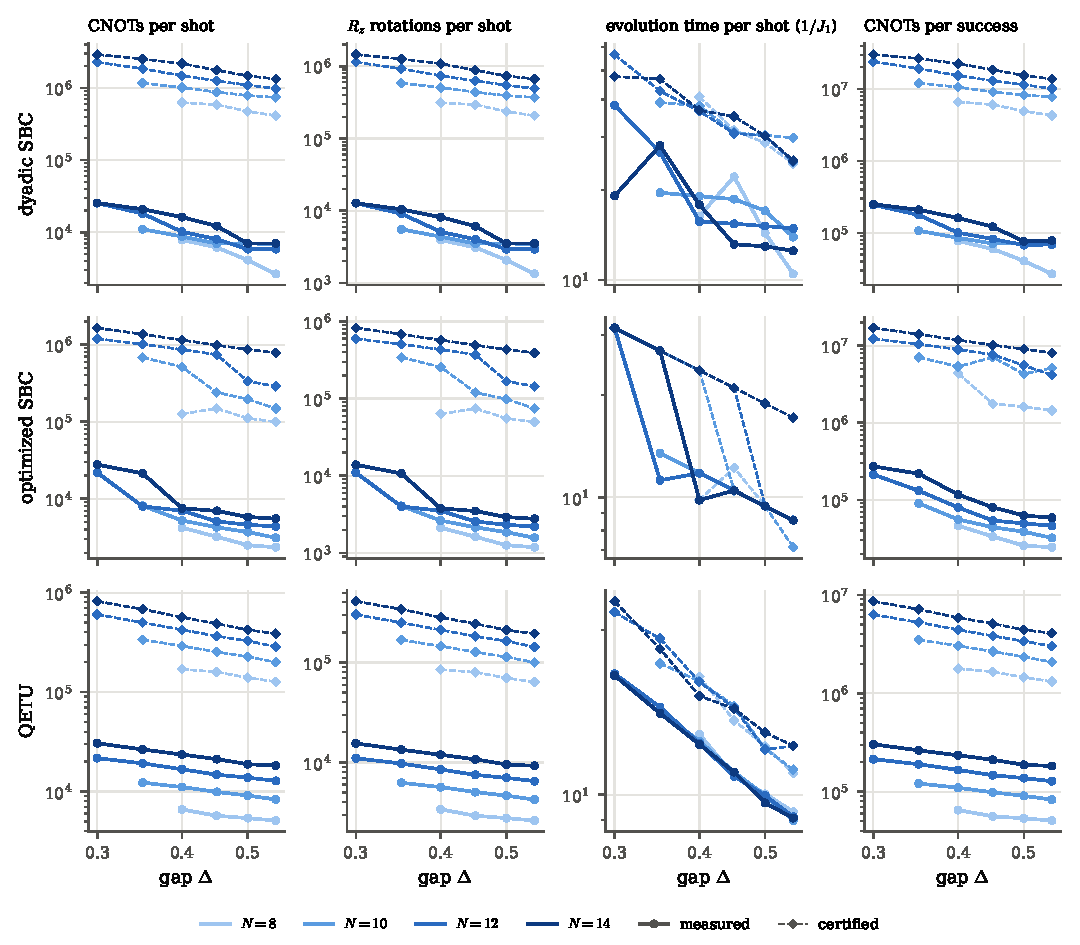
\includegraphics[width=\linewidth]{figs/fig_filter_B.pdf}
\caption{Filter-only resources at $\gamma=0.10$ and $\varepsilon=10^{-3}$ against the gap, which is held fixed
across $N$. Layout as Fig.~\ref{fig:A}.}\label{fig:B}
\end{figure}

Closing the gap from 0.55 to 0.30 (a factor of 1.8) at $\gamma=0.1$, for $N=12$ and 14 and all $\varepsilon$:
\begin{center}\small
\begin{tabular}{lcc}\toprule
 & CNOTs (and $R_z$) per shot & evolution time per shot \\\midrule
dyadic, measured & 2.7--4.4$\times$ & 1.5--2.8$\times$ \\
QETU, measured & 1.7--1.9$\times$ & 1.8--2.1$\times$ \\
dyadic, certified & 2.2--2.6$\times$ & 1.7--2.3$\times$ \\
QETU, certified & 2.0--2.1$\times$ & 1.8--2.0$\times$ \\
\bottomrule\end{tabular}
\end{center}
The evolution time grows about as fast as $1/\Delta$ (1.8$\times$), which is the uncertainty-principle cost of
resolving a smaller gap. For QETU, the measured times for different $N$ lie on top of one another
(Fig.~\ref{fig:B}, third column). Once the gap is fixed in absolute units, the filter's length does not care how
big the system is.

The dyadic measured CNOTs grow faster than its time (up to 4.4$\times$). With a larger gap, its Trotter step can
be coarser, and that advantage is lost as the gap closes (Section~\ref{sec:mech}).

Per success at fixed $\gamma$, the picture is the same as per shot, because $p\approx\gamma$ does not depend
on $\Delta$.

\section{Mechanism: filter length, Trotter step, and gates}\label{sec:mech}

\begin{figure}[h]\centering
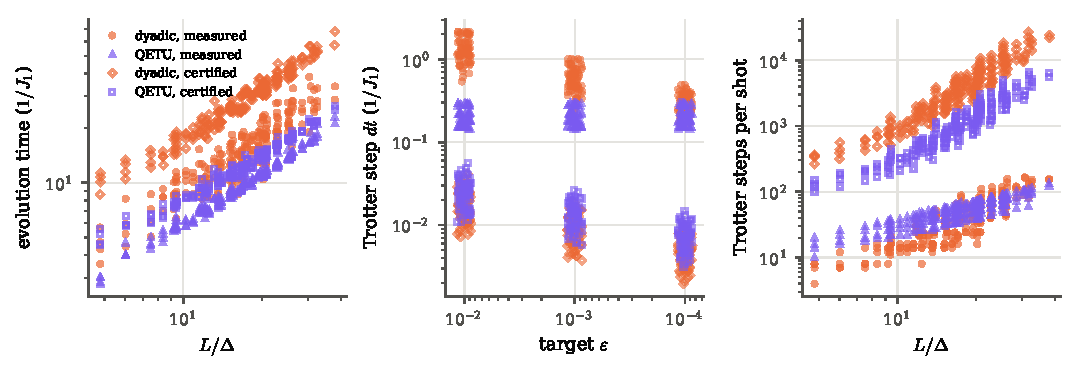
\includegraphics[width=\linewidth]{figs/fig_filter_mech.pdf}
\caption{All 222 cases. (a) Evolution time against $L/\Delta$. (b) Trotter step against $\varepsilon$
(jittered horizontally). (c) Trotter steps per shot against $L/\Delta$. Filled: measured. Open: certified.}
\label{fig:mech}
\end{figure}

The per-shot cost factorises as
\begin{equation}
\text{CNOTs per shot}\;=\;\underbrace{\frac{T}{dt}}_{\text{Trotter steps}}\times\underbrace{c_\text{step}(N)}_{\text{CNOTs per step}},
\qquad
\text{CNOTs per success}=\frac{\text{CNOTs per shot}}{p},\quad p\approx\gamma,
\end{equation}
and each factor depends on a different input:
\begin{itemize}
\item \textbf{Filter length $T$} depends on $\Delta$ and $L$ only (Fig.~\ref{fig:mech}a). Both filters, measured
and certified, follow $T\approx c\,L^{0.7\text{--}0.9}/\Delta^{1.0\text{--}1.2}$, with no $N$ dependence
(Table~\ref{tab:fit}). Measured QETU uses 0.65$\times$ the evolution time of the dyadic filter. The certified
times are close to the measured ones.
\item \textbf{Trotter step $dt$} depends on $\varepsilon$ and, for the dyadic filter, on $\Delta$
(Fig.~\ref{fig:mech}b).
  \begin{itemize}
  \item The measured dyadic filter tolerates very coarse steps: median $dt=1.25$, 0.56, 0.30 (in $1/J_1$) at
  $\varepsilon=10^{-2},10^{-3},10^{-4}$, growing roughly as $\varepsilon^{0.3}\Delta^{1.2}$.
  \item Measured QETU always needs exactly one Strang step per query, so $dt=\tau/W$ (0.15--0.29).
  \item The certified steps are about 60--75$\times$ finer than the measured dyadic ones: median $dt=0.017$, 0.009, 0.005 for dyadic. They also
  shrink as the total time grows, because the a-priori bound must cover the whole evolution.
  \end{itemize}
  This is why the certified step count grows as $L^{1.8\text{--}2.0}$, against $L^{0.7\text{--}0.9}$ measured
  (Fig.~\ref{fig:mech}c).
\item \textbf{CNOTs per step} grow linearly in $N$ (median 41$N$ for this two-neighbour chain), and
$R_z=0.25\times$CNOTs.
  \begin{itemize}
  \item For QETU, the steps per shot also grow as $N$, because $dt=\tau/W$ and $W\propto N$. So its CNOTs grow as
  $N^{2}$.
  \item The measured dyadic step count barely grows with $N$, so its CNOTs grow as about $N^{1.3}$.
  \end{itemize}
  The dyadic filter's coarser steps more than make up for its longer time: measured QETU needs 1.40$\times$
  the dyadic steps (median).
\end{itemize}

\begin{table}[h]\centering\small
\caption{Per-shot fits $X\approx a\,N^{\alpha}\Delta^{-\beta}L^{\lambda}\varepsilon^{-e}$ over all cases.
``rms''/``max'' are the typical and worst factor between a case and the fit. The $dt$ rows have the opposite
sign convention: a negative $\beta$ means $dt$ grows with the gap.}\label{tab:fit}
\begin{tabular}{lccccccc}\toprule
 & $a$ & $\alpha$ ($N$) & $\beta$ ($\Delta$) & $\lambda$ ($L$) & $e$ ($\varepsilon$) & rms & max \\\midrule
\multicolumn{8}{l}{\emph{dyadic, measured, per shot}} \\
\quad evolution time & $1.56$ & -0.24 & 1.19 & 0.77 & 0.04 & 1.18 & 1.5 \\
\quad Trotter step $dt$ & $3.88\times10^{1}$ & -0.40 & -1.22 & -0.00 & -0.32 & 1.24 & 2.5 \\
\quad Trotter steps & $2.27\times10^{-1}$ & 0.08 & 1.90 & 0.71 & 0.27 & 1.19 & 1.8 \\
\quad CNOTs & $5.98$ & 1.27 & 1.90 & 0.71 & 0.26 & 1.19 & 1.9 \\
\quad $R_z$ & $1.53$ & 1.26 & 1.89 & 0.71 & 0.26 & 1.19 & 1.9 \\
\multicolumn{8}{l}{\emph{QETU, measured, per shot}} \\
\quad evolution time & $8.35\times10^{-1}$ & -0.10 & 1.10 & 0.86 & 0.01 & 1.04 & 1.2 \\
\quad Trotter step $dt$ & $2.63$ & -1.12 & 0.13 & -0.00 & 0.00 & 1.01 & 1.0 \\
\quad Trotter steps & $3.17\times10^{-1}$ & 1.02 & 0.96 & 0.86 & 0.01 & 1.04 & 1.2 \\
\quad CNOTs & $8.45$ & 2.20 & 0.96 & 0.86 & 0.01 & 1.04 & 1.2 \\
\quad $R_z$ & $2.27$ & 2.18 & 0.96 & 0.86 & 0.01 & 1.04 & 1.2 \\
\multicolumn{8}{l}{\emph{dyadic, certified, per shot}} \\
\quad evolution time & $1.81$ & 0.04 & 1.10 & 0.84 & 0.01 & 1.07 & 1.2 \\
\quad Trotter step $dt$ & $1.65$ & -0.81 & -0.20 & -1.20 & -0.11 & 1.15 & 1.6 \\
\quad Trotter steps & $1.09$ & 0.85 & 1.30 & 2.03 & 0.12 & 1.16 & 1.8 \\
\quad CNOTs & $2.81\times10^{1}$ & 2.04 & 1.30 & 2.03 & 0.12 & 1.16 & 1.8 \\
\quad $R_z$ & $7.04$ & 2.04 & 1.30 & 2.03 & 0.12 & 1.16 & 1.8 \\
\multicolumn{8}{l}{\emph{QETU, certified, per shot}} \\
\quad evolution time & $1.14$ & 0.01 & 1.00 & 0.73 & 0.01 & 1.04 & 1.2 \\
\quad Trotter step $dt$ & $1.87$ & -0.80 & -0.15 & -1.11 & -0.11 & 1.16 & 1.6 \\
\quad Trotter steps & $6.10\times10^{-1}$ & 0.81 & 1.14 & 1.84 & 0.12 & 1.16 & 1.6 \\
\quad CNOTs & $1.57\times10^{1}$ & 2.00 & 1.14 & 1.84 & 0.12 & 1.16 & 1.6 \\
\quad $R_z$ & $3.97$ & 2.00 & 1.14 & 1.83 & 0.12 & 1.16 & 1.6 \\
\bottomrule\end{tabular}
\end{table}

\begin{table}[h]\centering\small
\caption{Per-success fits $X/p\approx a\,N^{\alpha}\Delta^{-\beta}L^{\lambda}\varepsilon^{-e}\gamma^{-g}$. $L$, $\varepsilon$
and $\gamma$ are correlated ($L$ is built from the other two), so read the three exponents together. The $1/\gamma$
from repetition shows up as $g\approx1$.}\label{tab:succ}
\begin{tabular}{llccccccc}\toprule
 & & $a$ & $\alpha$ & $\beta$ & $\lambda$ & $e$ & $g$ & rms \\\midrule
dyadic, measured & CNOTs & $5.52$ & 1.37 & 1.70 & 0.92 & 0.22 & 0.94 & 1.19 \\
dyadic, measured & $R_z$ & $1.41$ & 1.37 & 1.70 & 0.92 & 0.22 & 0.94 & 1.19 \\
dyadic, measured & time & $1.43$ & -0.13 & 1.00 & 0.99 & -0.01 & 0.94 & 1.18 \\
\addlinespace
QETU, measured & CNOTs & $8.30$ & 2.21 & 0.95 & 0.85 & 0.01 & 1.00 & 1.04 \\
QETU, measured & $R_z$ & $2.23$ & 2.18 & 0.95 & 0.85 & 0.01 & 1.00 & 1.04 \\
QETU, measured & time & $8.22\times10^{-1}$ & -0.09 & 1.08 & 0.84 & 0.01 & 1.00 & 1.04 \\
\addlinespace
dyadic, certified & CNOTs & $5.75\times10^{1}$ & 2.05 & 1.32 & 1.06 & 0.24 & 1.27 & 1.05 \\
dyadic, certified & $R_z$ & $1.44\times10^{1}$ & 2.05 & 1.32 & 1.06 & 0.24 & 1.27 & 1.05 \\
dyadic, certified & time & $2.31$ & 0.04 & 1.10 & 0.74 & 0.00 & 1.03 & 1.09 \\
\addlinespace
QETU, certified & CNOTs & $3.26\times10^{1}$ & 2.01 & 1.17 & 0.83 & 0.24 & 1.28 & 1.04 \\
QETU, certified & $R_z$ & $8.22$ & 2.01 & 1.17 & 0.83 & 0.24 & 1.28 & 1.04 \\
QETU, certified & time & $1.43$ & 0.01 & 1.00 & 0.65 & 0.00 & 1.02 & 1.05 \\
\bottomrule\end{tabular}
\end{table}

\section{Discussion}

\paragraph{Depth versus shots.} The two inputs act on different resources:
\begin{itemize}
\item The gap controls the coherent part of the computation: evolution time, Trotter steps, and therefore circuit
depth, CNOTs and $R_z$ per shot. On hardware where depth is the binding limit (coherence time, or the error budget
of one logical circuit), the gap decides whether the filter fits at all.
\item The trial overlap controls mainly the number of repetitions. A poor trial does not make the circuit much
deeper, it makes you run it more often.
\end{itemize}
Improving the trial state therefore buys shots, while a larger gap (or a sharper filter) buys depth.

\paragraph{Why the overlap is only logarithmic per shot.} A filter of length $T$ suppresses every state above the
gap by roughly $e^{-c\,T\Delta}$. Reaching infidelity $\varepsilon$ from a trial with excited weight $1-\gamma$ needs
suppression $\eta^2=\gamma\varepsilon/(1-\gamma)$, hence $T\propto\ln(1/\eta)/\Delta\propto L/\Delta$. The overlap is
inside the log; the gap is not.

\paragraph{Why the certificate is expensive, and where to fix it.} The certificate already sizes the filter
length close to what simulation needs (1.3--2$\times$). Its 20--90$\times$ excess in gates comes from the Trotter
step. Two consequences follow:
\begin{itemize}
\item Tighter commutator bounds, or a posteriori Trotter error estimates, would recover most of the gap between
certified and measured cost. A better filter design would not.
\item The certified CNOTs grow as $L^{2}$ rather than $L$, so the certificate penalises poor trials and tight
$\varepsilon$ more than the physics does.
\end{itemize}

\paragraph{Dyadic versus QETU.} QETU needs less evolution time, but it must take one fine Strang step per short
query. The dyadic pulses are long and smooth enough that the measured Trotter error stays below $\varepsilon$
at steps of order $1/J_1$. At $\varepsilon=10^{-4}$ that advantage shrinks ($dt$ falls as $\varepsilon^{0.3}$),
which is where QETU becomes the cheaper filter.

\paragraph{Caveats.} $N=8$--14 and $\Delta=0.30$--0.55 are narrow ranges, so the exponents describe these data
and are not asymptotic laws. $R_z$ counts are arbitrary-angle rotations, before any synthesis into Clifford$+T$.
The time is Hamiltonian evolution time; it is not wall-clock time on a device.

\end{document}
